% Chapter 16: Linear response of the rates and the pair formula. Sources: misc/reviews/nick-volume3/vol3/chD_progress.tex 15-31, 35-63, 65-180, 186-243, 245-280, 282-326 (status table kept) and chC_path_detail.tex 100-121, 135-170 (condensed into the introduction); reports U12 M1 to M6, M8, M9, M11 and minors; verification W3 V15. Date 17 Nov 2026.
\label{ch:progress}

This chapter reports on the first steps along route B, the rates of the chain of the zeros (Chapter~\ref{b:ch:chain}). It contains one proved formula for the derivative of every rate with respect to every zero (Theorem~\ref{pp:thm:lr}), floating point computations built on it, a classical rank update for the Hankel determinants with an added pair of atoms, and an experiment in which a pair of zeros of $\zeta$ is collided and pushed off the line. The experiments and the draft are from an unrefereed note of Polson (November 2026).

\section{What route B asks}\label{pp:sec:intro}

The criterion for RH is on the power sums $s_n$ of the zeros, which are the Taylor coefficients of $G'/G$, the logarithmic derivative. They are to the Taylor coefficients of $G$ what cumulants are to moments. Hankel determinants of moments of a positive measure are positive for free, since they are integrals of a squared Vandermonde determinant. Taking a logarithm destroys that positivity, and the problem is to recover it. Cumulants have a positivity theory in one classical situation, an infinitely divisible law, where they are moments of the L\'evy measure. That is the Thorin representation on which the programme of these volumes is built.

By Krein's theory the measure of the zeros is the spectral measure of a unique vibrating string, and the continued fraction is its discrete form (Section~\ref{bk:sec:string}). In every solved model the string is known in advance, as a diffusion: Brownian motion on an interval for the cosine, Bessel processes for Bessel functions. A proof by route B would exhibit the string of $\xi$, or a positive recurrence for its rates, without reference to the zeros. The smooth part is understood: the gamma factor alone gives a chain with rates $\alpha^\Gamma_j$ (the rates of the chain of the smooth zeros, Chapter~\ref{b:ch:chain}, which follow the law \eqref{eq:ch21:ratelaw}; the law is heuristic, and Chapter~\ref{l:ch:bohr} proves its direct half to leading order), and the true rates are $\alpha_j=\alpha_j^\Gamma(1+\varepsilon_j)$ with a fluctuation $\varepsilon_j$ that is small wherever it has been computed. A semiclassical candidate for $\varepsilon_j$ as a sum over primes was derived in Chapter~\ref{b:ch:chain} and rejected by computation. The steps, in order of ambition, are these.
\begin{enumerate}
\item The inverse half of the law: the chain of the smooth zeros has the rates of the law \eqref{eq:ch21:ratelaw} to leading order. This is a stability statement for the map from a spectral measure to its rates and does not involve the primes.
\item Linear response: the first order change of $\log\alpha_j$ when one zero moves. Its shape decides whether the fluctuation at level $j$ depends on a few zeros near the turning height or on many.
\item The pair formula: what a conjugate pair of zeros off the line does to the Hankel determinants and the rates, and why each pair costs exactly two negative rates.
\item The chain across a collision: as two zeros of $\zeta$ approach, merge and leave the line, which is what the backward heat flow does to a close pair in the isolated pair model, what does the chain see, and when?
\item A solved model that is not classical, with fluctuating zeros, in which positivity of all rates is proved by a structural argument; and, last, a positive formula for the rates of $\xi$, which is RH.
\end{enumerate}
Steps 2 to 4 are taken up here: step 2 is computed from an exact formula, step 3 is reduced to one sign change of each update determinant, and step 4 is computed for one isolated pair. Step 1 is stated as a conjecture with evidence (Conjecture~\ref{pp:conj:norm}), and step 5 is open. A milestone is worth setting if either outcome teaches something: if the response were not local, the fluctuation could not be read from the zeros near the turning height, and the chapter shows that it is not.

Throughout, the atoms of the measure of the zeros are $x_\gamma=1/\gamma^2$, $\nu=\sum_\gamma x_\gamma\delta_{x_\gamma}$ is the measure of Section~\ref{t:sec:moments}, $h_n$ is the squared norm of the $n$th monic orthogonal polynomial $p_n$ of $\nu$, and $h'_n$, $p'_n$ are the same objects for the measure $x\,\nu$. The rates are the numbers $c_j$ of Section~\ref{sec:ch21:hankel}, written $\alpha_j$ here, and in this notation
\begin{equation}\label{pp:eq:ratesh}
\alpha_{2n}=\frac{h_n}{h'_{n-1}},\qquad \alpha_{2n+1}=\frac{h'_n}{h_n},
\end{equation}
which is the determinant formula of Section~\ref{t:sec:moments} rewritten with $h_n=\Delta_{n+1}/\Delta_n$ and $h'_n=\Delta'_{n+1}/\Delta'_n$. (The draft of the note uses atoms $2/\gamma^2$ and rates twice as large, and the numbers below have been converted.)

\section{Linear response}\label{pp:sec:lr}

\subsection{An exact formula}

\begin{theorem}[Linear response of the rates]\label{pp:thm:lr}
Let $\nu=\sum_kw_k\delta_{x_k}$ be a positive discrete measure with infinitely many atoms, and suppose the weight of each atom is a differentiable function $w_k=w(x_k)$ of its position, with finite moments of $\nu$. Write $Q_{n,k}=\sqrt{w_k}\,p_n(x_k)/\sqrt{h_n}$. Then
\begin{equation}\label{pp:eq:lr}
\frac{\partial\log h_n}{\partial x_k}=Q_{n,k}^2\,\frac{w'(x_k)}{w(x_k)}-2\sum_{l\ne k}\frac{Q_{n,l}^2-Q_{n,l}Q_{n,k}\sqrt{w_l/w_k}}{x_l-x_k},
\end{equation}
and the same holds for $h'_n$ with $x\,w(x)$ in place of $w(x)$ and the polynomials of $x\,\nu$. The derivatives of $\log\alpha_j$ follow from \eqref{pp:eq:ratesh}.
\end{theorem}

\begin{proof}
The squared norm is a minimum, $h_n=\min\sum_lw_l\,p(x_l)^2$ over monic $p$ of degree $n$, attained at $p_n$. By the envelope theorem the derivative of the minimum is the partial derivative with the minimiser held fixed:
\[
\frac{\partial h_n}{\partial x_k}=\frac{\dd}{\dd x}\Big[w(x)\,p_n(x)^2\Big]_{x=x_k}=w'(x_k)p_n(x_k)^2+2w_kp_n(x_k)p_n'(x_k).
\]
Dividing by $h_n$ gives the first term of \eqref{pp:eq:lr} and $2w_kp_n(x_k)p_n'(x_k)/h_n$. For the latter, the divided difference $q(x)=(p_n(x)-p_n(x_k))/(x-x_k)$ is a polynomial of degree $n-1$, so $\sum_lw_lp_n(x_l)q(x_l)=0$. The term $l=k$ of this sum is $w_kp_n(x_k)p_n'(x_k)$, and moving the other terms across gives
\[
w_kp_n(x_k)p_n'(x_k)=-\sum_{l\ne k}w_lp_n(x_l)\,\frac{p_n(x_l)-p_n(x_k)}{x_l-x_k},
\]
which is the sum in \eqref{pp:eq:lr} after division by $h_n$.
\end{proof}

Two remarks on the form. The quantities $Q_{n,k}$ are the components of the Lanczos vectors of the chain, which are computed stably, so the formula needs neither the zeros of $p_n$ nor a difference quotient. The naive form, with $p_n'/p_n$ written as a sum over the zeros of $p_n$, fails in floating point for exactly the atoms that matter: those well below the level, which $p_n$ has already resolved, so that a zero of $p_n$ coincides with the atom to machine precision while the product of a vanishing $Q_{n,k}^2$ and an infinite $p_n'/p_n$ is of order one. The orthogonality form avoids the product altogether.

For the zeros of $\zeta$ the atom at $x_k=1/\gamma_k^2$ has weight $w=x$, so $w'/w=1/x$ for $\nu$ and $2/x$ for $x\,\nu$, and $\partial/\partial\gamma_k=-(2x_k/\gamma_k)\,\partial/\partial x_k$. We write $J_{jk}=\partial\log\alpha_j/\partial\gamma_k$. These logarithmic derivatives do not depend on the normalisation of the rates.

\begin{computation}\label{pp:comp:check}
With $3000$ smooth zeros and a lumped tail, the Jacobian for levels $j\le999$ and zeros $k\le1200$ takes four seconds. Central differences with step $10^{-4}$ in $\gamma_k$, for $k=1,10,100,300$, agree with it to $2\times10^{-10}$, against entries of size up to $0.19$ (computed in floating point; not rerun).
\end{computation}
% UNVERIFIED: pp:comp:check, lr, range, universal, norm, rigid need the 6703 zeros; not rerun in W3 (V15).

\subsection{The fluctuation is a smooth functional of the displacements}

Let $\gamma_k^{\rm s}$ be the smooth zeros, defined by $\theta(\gamma)/\pi+1=k-\frac12$, and $\delta\gamma_k=\gamma_k-\gamma_k^{\rm s}$ the displacements of the true zeros. For the first $6703$ zeros the displacement, measured in mean spacings, has standard deviation $0.27$ and never exceeds $0.86$.
% TODO (R_response M12): sd 0.27 from variance 0.075 of the later section; nc_v3_spins.tex says 0.28, neither rerun on the 6703 zeros. Recompute and print one value. Let $\alpha_j^{\rm s}$ be the rates of the chain of the smooth zeros, and
\[
\lambda_j=\log\frac{\alpha_j}{\alpha^{\rm s}_j}.
\]
The chain of the smooth zeros is the Gamma chain of Chapter~\ref{b:ch:chain}, so $\alpha^{\rm s}_j=c^\Gamma_j$ and $\lambda_j=\log(1+\varepsilon_j)$, which is defined exactly when $\alpha_j>0$. Along the straight path $\gamma(\tau)=\gamma^{\rm s}+\tau\,\delta\gamma$, $0\le\tau\le1$, every configuration is real and ordered, since a convex combination of two increasing sequences is increasing. So the chain exists along the whole path, and
\begin{equation}\label{pp:eq:path}
\lambda_j=\int_0^1\sum_kJ_{jk}\big(\gamma(\tau)\big)\,\delta\gamma_k\,\dd\tau
\end{equation}
exactly. The question is how much of this integral is captured by simple rules.

\begin{computation}\label{pp:comp:lr}
With all $6703$ known zeros and $10000$ zeros in all, for levels $j\le1999$:
\begin{center}\small
\begin{tabular}{@{}lccc@{}}
\toprule
levels & spread of $\lambda_j$ & first order at $\gamma^{\rm s}$ & Simpson rule on \eqref{pp:eq:path}\\
\midrule
$1$ to $100$ & $0.069$ & $0.900$ & $0.99999$\\
$100$ to $500$ & $0.037$ & $0.786$ & $0.99984$\\
$500$ to $1000$ & $0.024$ & $0.748$ & $0.99931$\\
$1000$ to $1500$ & $0.020$ & $0.656$ & $0.99649$\\
$1500$ to $1999$ & $0.016$ & $0.676$ & $0.99917$\\
all & $0.029$ & $0.789$ & $0.99934$\\
\bottomrule
\end{tabular}
\end{center}
The middle columns are coefficients of determination, the share of the variance of $\lambda_j$ explained. The Simpson rule uses the Jacobian at $\tau=0,\frac12,1$, and its largest error at any level is $0.0096$ (computed in floating point).
\end{computation}

\begin{figure}[ht]
\centering
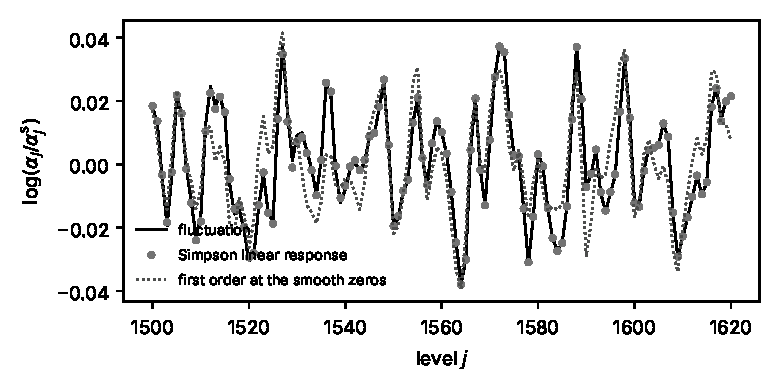
\includegraphics[width=\textwidth]{fig/v3/pp_fig_lr.pdf}
\caption{The fluctuation $\lambda_j$ of the chain of $\zeta$ on levels $1500$ to $1620$, the Simpson rule for \eqref{pp:eq:path}, and the first order prediction at the smooth zeros.}\label{pp:fig:lr}
\end{figure}

Chapter~\ref{b:ch:chain} suggested, from a regression on the displacements of the $25$ zeros nearest the turning height, that the fluctuation is predominantly a local and nonlinear function of those zeros (a suggestion that chapter now calls superseded). Computation~\ref{pp:comp:lr} corrects half of that conclusion and sharpens the other half. The fluctuation is not essentially nonlinear: first order response explains four fifths of it, and a three point rule along the path explains all but a thousandth. What the regression missed is the range of the response.

\begin{figure}[ht]
\centering
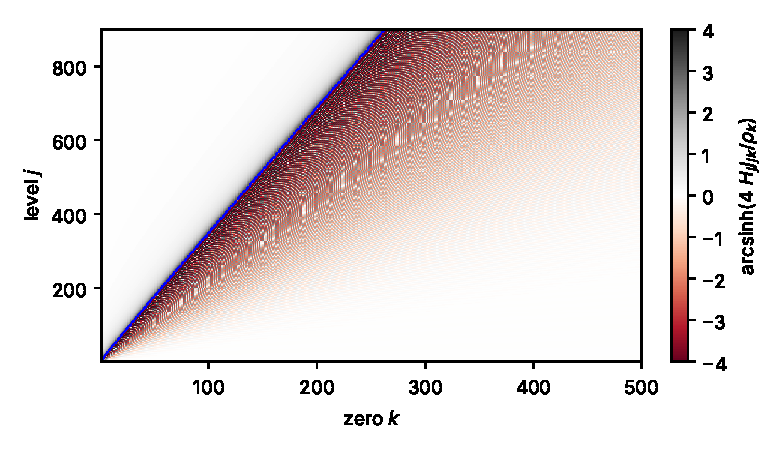
\includegraphics[width=\textwidth]{fig/v3/pp_fig_jac.pdf}
\caption{The Jacobian $J_{jk}$ of the rates with respect to the zeros, scaled by $H_j/\rho(\gamma_k)$ and compressed by an inverse hyperbolic sine, for levels $j\le900$ and zeros $k\le500$. The dashed line marks the first zero above the turning height of each level. To its left the response is small and smooth; to its right it is large and oscillates.}\label{pp:fig:jac}
\end{figure}

\subsection{The response is not local}

\begin{computation}\label{pp:comp:range}
For levels $100<j\le1999$, keep in the Simpson rule only the zeros within $m$ mean spacings of the turning height $H_j=(4\alpha^{\rm s}_j)^{-1/2}$. The share of variance explained is
\begin{center}\small
\begin{tabular}{@{}lccccccc@{}}
\toprule
$m$ & $2$ & $5$ & $10$ & $20$ & $40$ & $80$ & $160$\\
\midrule
share & $0.14$ & $0.31$ & $0.47$ & $0.63$ & $0.78$ & $0.89$ & $0.96$\\
\bottomrule
\end{tabular}
\end{center}
Keeping only the zeros below the turning height explains $3$ per cent of the variance at first order; keeping only those above it explains $73$ per cent, against $74$ per cent for both (computed in floating point).
\end{computation}

\begin{figure}[ht]
\centering
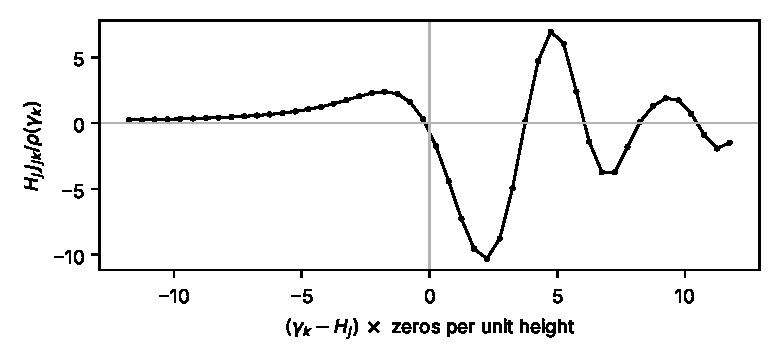
\includegraphics[width=\textwidth]{fig/v3/pp_fig_kernel.pdf}
\caption{The response kernel in scaled form, averaged over levels $300$ to $900$: $H_jJ_{jk}$ divided by the density $\rho(\gamma)=\log(\gamma/2\pi)/2\pi$ of zeros, against the distance of $\gamma_k$ from the turning height in mean spacings.}\label{pp:fig:kernel}
\end{figure}

Figure~\ref{pp:fig:jac} shows the whole Jacobian and Figure~\ref{pp:fig:kernel} a scaled average of its rows. Below the turning height the kernel is positive, smooth and slowly decaying; above it, it oscillates, with a first trough two spacings above the turning height that is four times deeper than the peak below, and a period of about two spacings further out. A displacement field that oscillates from zero to zero, as the true displacements do, is almost invisible to the smooth part, so the oscillating part above the turning height carries the fluctuation.

This explains the failure of the candidate prime formula \eqref{b:eq:cand}. That formula came from the semiclassical inversion \eqref{b:eq:inv}, whose kernel is $(H^2-\gamma^2)^{-1/2}$ on $\gamma<H$: it sees only the zeros below the turning height, which is the part of the response that, by Computation~\ref{pp:comp:range}, carries three per cent of the signal. The correct kernel is the Jacobian, and its active part lies on the other side.

\subsection{The kernel is not special to the zeta function}

The shape in Figure~\ref{pp:fig:kernel} could be a property of $\zeta$ or a property of chains in general. The cosine model of Chapter~\ref{ch:cosine} decides between the two: its zeros are evenly spaced, its chain is Lambert's continued fraction with $\alpha_j=1/((2j-1)(2j+1))$, and its turning height at level $j$ is $H_j=\frac12\sqrt{(2j-1)(2j+1)}$.

\begin{computation}\label{pp:comp:universal}
With $4000$ zeros $(k-\frac12)\pi$ and a lumped tail, the Jacobian of Theorem~\ref{pp:thm:lr} for levels $j\le999$ and zeros $k\le1500$, scaled and averaged over levels $300$ to $900$ exactly as for $\zeta$, has correlation $0.998$ with the kernel of $\zeta$ over the window of $24$ mean spacings around the turning height. Its amplitude in the scaling of the figure is about twice that of $\zeta$, and most of the factor comes from the scaling by $H_j$, which at the same level is larger for the cosine by a factor that runs from about $1.4$ at level $300$ to about $1.8$ at level $900$. In the natural units, the response of $\log\alpha_j$ per mean spacing of displacement, the row norms are $1.09$, $1.09$ and $1.14$ at levels $200$, $500$ and $900$, against $0.99$ to $1.12$ for $\zeta$ (Computation~\ref{pp:comp:norm}; computed in floating point).
\end{computation}

\begin{figure}[ht]
\centering
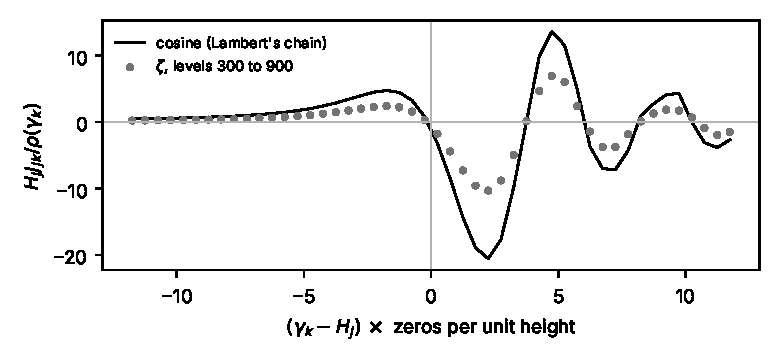
\includegraphics[width=\textwidth]{fig/v3/pp_fig_kernel2.pdf}
\caption{The scaled response kernel of the cosine model, whose chain is Lambert's continued fraction, and that of $\zeta$.}\label{pp:fig:kernel2}
\end{figure}

So the shape of the response kernel is a property of the chain of an increasing sequence with a smooth density, not of the arithmetic. Its scaled limit can be sought in the cosine model, where the orthogonal polynomials of the spectral measure are explicit: they are the denominators of Lambert's continued fraction, polynomials of Lommel type attached to Bessel functions of half integer order. This turns the second open problem below into a problem about classical special functions. It also gives a cleaner reading of route B: the arithmetic enters the fluctuation only through the displacements of the zeros, and it is filtered by a kernel close to the one of the cosine model, which is the chain of Brownian motion on an interval.

\subsection{Stability}

The inverse half of the law of Chapter~\ref{l:ch:bohr} is a stability statement for the map from a spectral measure to its rates. The Jacobian measures that stability directly. Let
\[
\|J_j\|=\sum_k\frac{|J_{jk}|}{\rho(\gamma_k)},
\]
the change in $\log\alpha_j$ per unit displacement of every zero by one mean spacing in the worst direction.

\begin{computation}\label{pp:comp:norm}
At the smooth zeros, $\|J_j\|$ lies between $0.99$ and $1.12$ for every level checked between $100$ and $1900$ (both parities): $1.12$ at $j=100$, $1.00$ at $200$, $1.10$ at $400$, $1.02$ at $700$, $1.07$ at $1000$, $1.05$ at $1300$, $0.99$ at $1600$ and $1.05$ at $1900$ (computed in floating point).
\end{computation}

So to first order, moving every zero by at most $\kappa$ mean spacings changes every rate by a factor between $e^{-1.12\kappa}$ and $e^{1.12\kappa}$, at every level checked between $100$ and $1900$. The observed fluctuation, of order $0.03$ against a displacement of order $0.3$ spacings, is ten times smaller than this bound, because the displacements oscillate and the kernel averages them.

\begin{conjecture}\label{pp:conj:norm}
$\sup_j\|J_j\|<\infty$ at the smooth zeros of $\zeta$, 
% TODO (R_response M11): the draft's general clause (any increasing sequence with gamma_k log gamma_k ~ 2 pi k and bounded displacements) was cut: the reference sequence and the density in the norm are undefined for a general sequence. Authors to state which.
\end{conjecture}

The conjecture is the linearised form of the inverse half of the law. It would be a statement on route B that is uniform in the level and does not involve the primes. Eight levels support it, and nothing more.

\subsection{The size of the fluctuation is not set by rigidity}

The zeros of $\zeta$ are rigid: by the theory of the pair correlation \cite{Montgomery73}, the count of zeros in a window fluctuates far less than it would for independent points. The displacements show this directly. Measured in mean spacings they have variance $0.075$ each, but the sum of $10$ consecutive displacements has variance $0.102$ and the sum of $100$ has variance $0.128$, where independent displacements would give $0.75$ and $7.5$. One might expect this rigidity to be the reason the fluctuation of the chain is small.

\begin{computation}\label{pp:comp:rigid}
On levels $200$ to $1998$ the first order response to the true displacements has standard deviation $0.0223$. The same displacements shuffled at random among the zeros give $0.0229$, averaged over $20$ shuffles, and independent normal displacements with the same variance give $0.0231$. The lag one correlation of the displacements is $0.008$ (computed in floating point).
\end{computation}

So rigidity plays no measurable role. The response is governed by the oscillating part of the kernel above the turning height, which is blind to sums of displacements over long windows, and the size of $\lambda_j$ is set by the variance of a single displacement and the $\ell^2$ norm of the kernel row. This has a consequence for any attempt to bound $\lambda_j$ from below: the relevant input is the distribution of individual displacements, that is of $S(t)$ at the zeros, and not the long range correlations that make the zeros a rigid system.

\section{The pair formula}\label{pp:sec:pair}

The second milestone asks what a pair of zeros off the line does to the chain. The answer is an exact identity for any number of added atoms. It is a form of the Uvarov transformation of a measure by point masses \cite{Uvarov69}, combined with the determinant identity for a low rank update, and is classical. We state it as a lemma because the rest of the section uses it in this form.

\begin{lemma}[Rank update, after Uvarov]\label{pp:thm:pair}
Let $\nu_0$ be a positive measure on $(0,\infty)$ with infinitely many points of support and finite moments, with orthonormal polynomials $\phi_m$, and let $\nu=\nu_0+\sum_{a=1}^rw_a\delta_{x_a}$ with atoms $x_a$ and weights $w_a$, real or complex. Write $W=\operatorname{diag}(w_a)$ and $K_n=\big[\sum_{m<n}\phi_m(x_a)\phi_m(x_b)\big]_{a,b}$, a symmetric matrix with no complex conjugation. Then for the Hankel determinants $\Delta_n=\det[s_{i+j}]_{i,j<n}$,
\[
\Delta_n(\nu)=\Delta_n(\nu_0)\,\det\big(I_r+WK_n\big).
\]
The same holds for $\Delta'_n$ with $x\,\nu_0$, its orthonormal polynomials, and weights $w_ax_a$. Writing $r_n$ and $r'_n$ for the two determinants,
\begin{equation}\label{pp:eq:ratio}
\alpha_{2n}=\alpha^0_{2n}\,\frac{r_{n+1}\,r'_{n-1}}{r_n\,r'_n},\qquad
\alpha_{2n+1}=\alpha^0_{2n+1}\,\frac{r_n\,r'_{n+1}}{r_{n+1}\,r'_n}.
\end{equation}
\end{lemma}

\begin{proof}
With $v(x)=(1,x,\dots,x^{n-1})^{\mathsf T}$ the moment matrix is $M_n(\nu)=M_n(\nu_0)+V\,W\,V^{\mathsf T}$, where $V$ has columns $v(x_a)$. By the determinant identity for a low rank update, $\det M_n(\nu)=\det M_n(\nu_0)\det(I_r+WV^{\mathsf T}M_n(\nu_0)^{-1}V)$, and $v(x)^{\mathsf T}M_n(\nu_0)^{-1}v(y)=\sum_{m<n}\phi_m(x)\phi_m(y)$ is the reproducing kernel of the polynomials of degree less than $n$. Both are polynomial identities in the atoms and weights, so they hold for complex values. Formula \eqref{pp:eq:ratio} follows from \eqref{pp:eq:ratesh}.
\end{proof}

\begin{corollary}\label{pp:cor:real}
If all added atoms are positive real numbers and all weights positive, then $r_n>0$ and $r'_n>0$ for every $n$.
\end{corollary}

\begin{proof}
$K_n$ is then a Gram matrix, so $I+W^{1/2}K_nW^{1/2}$ is positive definite and has the same determinant as $I+WK_n$.
\end{proof}

The corollary is the familiar fact that a positive measure has positive Hankel determinants, so it is no more than the Stieltjes positivity that is the starting point of Section~\ref{sec:ch21:hankel}. What the lemma adds is a factorisation: the whole contribution of a set of added atoms to every determinant, and so to every rate, is the explicit factor $r_n$.

For a single conjugate pair the determinant has a transparent form. Put $x_1=x$, $x_2=\bar x$, $w_1=w$, $w_2=\bar w$, and
\[
A_n=\sum_{m<n}|\phi_m(x)|^2,\qquad B_n=\sum_{m<n}\phi_m(x)^2 .
\]
Since the $\phi_m$ have real coefficients, $K_n=\begin{pmatrix}B_n&A_n\\A_n&\bar B_n\end{pmatrix}$, and
\begin{equation}\label{pp:eq:D}
\begin{aligned}
r_n&=\big|1+wB_n\big|^2-|w|^2A_n^2,\\
A_n^2-|B_n|^2&=2\sum_{m,l<n}\big(\Im\,\phi_m(x)\overline{\phi_l(x)}\big)^2 .
\end{aligned}
\end{equation}
The pair is harmless at level $n$ while $|1+wB_n|>|w|A_n$, and it makes $\Delta_n$ negative when the inequality is reversed. For a real pair the matrix $K_n$ is a Gram matrix and Corollary~\ref{pp:cor:real} applies, so no reversal is possible. For a complex pair $A_n$ grows without bound, because the measure is determinate and $x$ is not real, while $|B_n|$ falls behind $A_n$ at a rate set by the imaginary parts in \eqref{pp:eq:D}; once $|w|(A_n-|B_n|)$ exceeds one the sign is negative.

\begin{proposition}[Two negative rates]\label{pp:prop:two}
Suppose that for $N-3\le n\le N+1$ the sign of $r_n$ changes exactly once, between $N-1$ and $N$, and that the sign of $r'_n$ changes exactly once in the same range, between $N'-1$ and $N'$. Among the factors $\alpha_j/\alpha^0_j$ with $2N-4\le j\le2N+1$, if $N'=N$ the negative ones are exactly those of $\alpha_{2N-2}$ and $\alpha_{2N}$, and if $N'=N-1$ exactly those of $\alpha_{2N-3}$ and $\alpha_{2N-1}$. In particular, if the rates $\alpha^0_j$ are positive there, these are the only negative rates among them.
\end{proposition}

\begin{proof}
Insert the signs into \eqref{pp:eq:ratio}. For $N'=N$: the factor of $\alpha_{2N-2}$ is $r_Nr'_{N-2}/(r_{N-1}r'_{N-1})$, with signs $(-)(+)/((+)(+))$; that of $\alpha_{2N}$ is $r_{N+1}r'_{N-1}/(r_Nr'_N)$, with signs $(-)(+)/((-)(-))$; that of $\alpha_{2N-1}$ is $r_{N-1}r'_N/(r_Nr'_{N-1})$, with signs $(+)(-)/((-)(+))$; and every other factor has an even number of negative terms. The case $N'=N-1$ is the same computation shifted by one level.
\end{proof}

Chapter~\ref{b:ch:chain} observed that each pair of zeros off the line of the control costs exactly two negative rates, and supported this by a count of negative squares of a Hankel form. Proposition~\ref{pp:prop:two} reduces the observation, locally at each pair, to a single sign change of each of $r_n$ and $r'_n$, at the same or neighbouring levels, which is what the computation below shows.

\begin{computation}\label{pp:comp:control}
The control from its zeros (Davenport and Heilbronn \cite{DH36}; for its zeros off the line see \cite{Spira94,BSO07}). A scan of the real function $e^{i\theta(t)}f(\frac12+it)$ with step $0.02$ finds $304$ zeros of the Davenport and Heilbronn function on the critical line below height $420$. Together with the two known quadruples off the line this is $308$ zeros, against the smooth count; the count falls short by about two at each of seven further places, between heights $164$ and $413$, where further zeros off the line lie. As the base $\nu_0$ take the $304$ zeros on the line, smooth zeros above height $420$ and a lumped tail. Add the four atoms $x=1/(\gamma\pm id)^2$ for $(d,\gamma)=(0.30852,85.69935)$ and $(0.15083,114.16334)$ by Lemma~\ref{pp:thm:pair}, in $300$ digit arithmetic.
\begin{enumerate}
\item The negative rates are exactly $\alpha_{148},\alpha_{150},\alpha_{217},\alpha_{219}$, the four levels found by the kernel route of Computation~\ref{b:comp:dh} at $1100$ and $1400$ digits. Here $r_n$ and $r'_n$ both turn negative at $n=75$, so Proposition~\ref{pp:prop:two} applies with $N=N'=75$ for the first pair and gives levels $148$ and $150$. The second pair makes each of them change sign again, near $n=110$, and the same local statement applies there (with $N=110$, $N'=109$) and gives levels $217$ and $219$.
\item The values are $\alpha_{148}=-9.5\times10^{-6}$, $\alpha_{150}=-3.4\times10^{-4}$, $\alpha_{217}=-6.0\times10^{-6}$, $\alpha_{219}=-1.7\times10^{-4}$, against $-8.9\times10^{-6}$, $-3.6\times10^{-4}$, $-4.0\times10^{-6}$, $-2.6\times10^{-4}$ from the kernel. The differences presumably come from the zeros off the line above height $164$, which the base omits.
\end{enumerate}
\end{computation}
% UNVERIFIED: levels 148, 150, 217, 219 and the values (W3 V15 did not rerun the pair formula levels); values are the draft's halved to the book normalisation.

The levels are read correctly from the zeros, by a formula that isolates the contribution of each pair, although the values differ from those of the kernel route by up to a factor of $1.5$. In particular, the failure of the control is entirely the failure of $r_n$ and $r'_n$: the real zeros, however they are arranged, contribute a positive factor.

\section{Collisions}\label{pp:sec:coll}

In the isolated pair model of the backward heat flow, a pair of neighbouring zeros approaches, collides and leaves the line, and the pairs that are close at $t=0$, the Lehmer pairs, do so first (heuristic: Rodgers and Tao \cite{RodgersTao} prove that $H_t$ has nonreal zeros for every $t<0$, not that each close pair collides). If RH failed, a zero off the line would be the end state of such a collision. So the question of how the chain responds to a collision is the question of how close to failure a configuration of real zeros can look.

The experiment holds all zeros of $\zeta$ fixed except one pair. Among the first $300$ zeros the closest pair, in units of the mean spacing, is $\gamma_{212}=415.018810$, $\gamma_{213}=415.455215$, with gap $0.4364$, or $0.29$ mean spacings. The pair is first brought together symmetrically about its centre $c=415.237$, then merged, and then pushed off the line to $c\pm i\eta$. For an isolated pair the heat flow of Section~\ref{sec:ch21:flow} does exactly this: in ordinate units the difference $\Delta$ of the two zeros satisfies $\dd\Delta/\dd t=1/\Delta$, so $\Delta^2=0.4364^2+2t$, the collision is at $t^*=-0.0952$, and for $t<t^*$ the pair is $c\pm i\eta$ with $\eta=\sqrt{(t^*-t)/2}$. All rates come from Lemma~\ref{pp:thm:pair} with the other zeros as base. The turning height of the chain reaches the pair at about level $715$.
% TODO (R_response minor): level 715 unverified and undefined: say whether the law, the smooth chain or the chain with the pair is meant; the smooth chain first exceeds 415.24 near level 708.
% UNVERIFIED: level 715 (not rerun). t* = -0.0952 confirmed in W3 V15; draft had -0.0238 (factor 4).

\begin{computation}\label{pp:comp:coll}
\begin{enumerate}
\item Real phase. With the gap reduced to $0.5$ times its true value, every rate stays positive and on the $120$ levels around level $715$ the largest change in any rate is $2.3$ per cent of its value. At complete merger the largest change is $9.1$ per cent and the smallest ratio of a rate to its value at the true gap is $0.91$ (computed in floating point; rerun with the first $376$ zeros).
\item Complex phase. For every $\eta$ from $0.5$ to $10^{-6}$ there are exactly two negative rates, two levels apart. The first is at level
\begin{center}\small
\setlength{\tabcolsep}{3pt}\begin{tabular}{@{}lcccccccccc@{}}
\toprule
$\eta$ & $0.5$ & $0.2$ & $0.1$ & $0.05$ & $0.02$ & $0.01$ & $10^{-3}$ & $10^{-4}$ & $10^{-5}$ & $10^{-6}$\\
\midrule
level & $693$ & $721$ & $726$ & $732$ & $738$ & $742$ & $751$ & $760$ & $768$ & $776$\\
\bottomrule
\end{tabular}
\end{center}
For $\eta\le0.02$ the level is $722.5+9.1\log_{10}(1/\eta)$ to within $1.5$ levels (computed in floating point; the levels at $\eta=0.5$, $0.2$, $0.05$, $10^{-3}$ and $10^{-6}$ were reproduced exactly).
\end{enumerate}
\end{computation}
% UNVERIFIED: levels for eta = 0.1, 0.02, 0.01, 1e-4, 1e-5 (not rerun). Draft items for gaps 0.2, 0.1, 0.01 (4.6, 5.7, 15 per cent) dropped: inconsistent with continuity (U12 M2), not rerun.

\begin{figure}[ht]
\centering
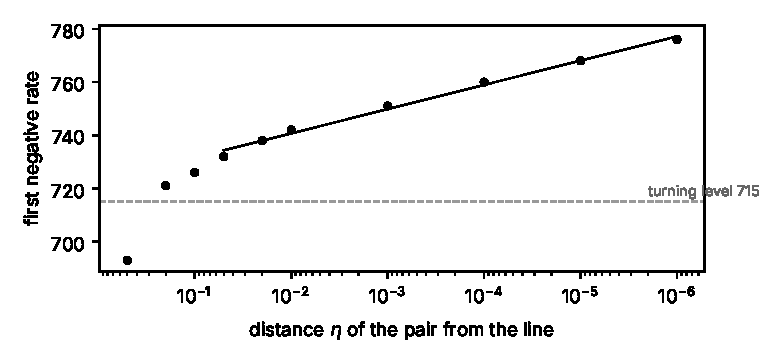
\includegraphics[width=\textwidth]{fig/v3/pp_fig_collision.pdf}
\caption{The first negative rate of the chain of $\zeta$ when the pair $\gamma_{212},\gamma_{213}$ is replaced by $c\pm i\eta$, against $\eta$. The dashed line is the level at which the turning height reaches the pair.}\label{pp:fig:coll}
\end{figure}

Three conclusions follow.

\paragraph{The margin is not consumed by approach.} A pair of zeros at distance $0.29$ mean spacings, then at distance zero, moves the rates near its level by less than ten per cent. The fluctuation $\varepsilon_j$ does not drift toward $-1$ as two zeros approach a collision, so no lower bound for $\varepsilon_j$ can be expected to become tight near a Lehmer pair. The near collisions of $\zeta$ are not near failures of the chain.

\paragraph{The failure is sharp and certain.} Once the pair is off the line the chain detects it at every distance tried, down to $10^{-6}$, always with exactly two negative rates, in agreement with Proposition~\ref{pp:prop:two}. In heat time, a pair that collided at $t^*$ is seen at time $t<t^*$ at a level that grows by about $4.6$ levels for each factor of ten in $t^*-t$.

\paragraph{The cost of a near miss is logarithmic.} The depth at which a pair is caught grows like $\log(1/\eta)$, about nine levels per factor of ten beyond the turning level. In \eqref{pp:eq:D} this is the statement that $A_n-|B_n|$ grows geometrically past the turning point, by a factor of about $10^{2/4.55}=2.75$ per index $n$, that is $1.66$ per level, since $A_n-|B_n|$ is of order $\eta^2$ at fixed $n$. The chain therefore resolves the distance from the line far more efficiently than the ladder of the density, where the corresponding failure appears at shifts of order $1/\eta$ and in minors of size $e^{-c/\eta}$ (Corollary~\ref{p:cor:scale}).

\section{What this changes on the path}\label{pp:sec:status}

\paragraph{The arithmetic enters through a known linear filter.} The fluctuation is the image of the displacements under a smooth, nearly linear map whose kernel is computed exactly by Theorem~\ref{pp:thm:lr}. Since the displacements are $-S(\gamma_k)/\rho(\gamma_k)$ to first order, $\lambda_j$ is, to the same order, a weighted sum of $S$ at about a hundred zeros above the turning height. The primes enter only through $S$. This is the linear response formula that the programme of Chapter~\ref{b:ch:chain} asked for. It does not bound $\lambda_j$, because $S$ is unbounded, but it replaces the search for a prime formula with a question about one explicit kernel.

\paragraph{The inverse half has a linear form.} Computation~\ref{pp:comp:norm} shows the response of the rates to the zeros bounded at the levels checked, in the natural units. Conjecture~\ref{pp:conj:norm} states this for all levels, and its proof would be the linearised inverse half of the law.

\paragraph{What would change the assessment.} Signs that a route is opening: a closed form or a sign preserving recurrence for the rates of a function with fluctuating zeros; a formula for the fluctuation that is exact at first order and tested on the control; any inequality for $\xi$ that is sharp along the heat flow and false for the control at the correct height. Signs that the path is closed: a proof that the fluctuation is unbounded below along some sequence for functions in a class that contains $\xi$; a demonstration that the map from zeros to rates is so unstable that no formula in terms of smooth data can control it; or a second control, with an Euler product of a weaker kind, that passes every structural test the chain can pose and still has zeros off the line. Further finite computation in agreement with RH would not change it, since it is shared by the control up to the height of its first bad zero.

\begin{table}[ht]
\centering\small
\caption{The milestones of route B after this chapter.}\label{pp:tab:status}
\begin{tabular}{@{}p{0.08\textwidth}p{0.34\textwidth}p{0.46\textwidth}@{}}
\toprule
route & milestone & status\\
\midrule
B & linear response of the rates to one zero & proved: exact formula (Theorem~\ref{pp:thm:lr}); response computed to be smooth, not local, carried by the zeros above the turning height\\[2pt]
B & inverse half of the law & linear form stated (Conjecture~\ref{pp:conj:norm}) and computed at eight levels up to $1900$\\[2pt]
B & two negative rates per pair & proved from one local sign change of $r_n$ and of $r'_n$ (Proposition~\ref{pp:prop:two}); the control read from its zeros (computed)\\[2pt]
C & the chain across a collision & computed for an isolated pair: blind to approach, certain after, depth logarithmic in $\eta$\\[2pt]
B & all rates positive in one nonclassical model & open\\
\bottomrule
\end{tabular}
\end{table}

\section{Open problems}\label{pp:sec:open}

\begin{openproblem}
Prove Conjecture~\ref{pp:conj:norm}. A route: the Lanczos vectors $Q_{n,k}$ have a WKB form with a turning point at $\gamma_k=H_n$, and the sum in \eqref{pp:eq:lr} can then be estimated by stationary phase.
\end{openproblem}

\begin{openproblem}
Find the scaled limit of the response kernel of Figure~\ref{pp:fig:kernel}. By Computation~\ref{pp:comp:universal} it can be computed in the cosine model, from the polynomials of Lambert's continued fraction. Its oscillation above the turning height suggests an Airy function of the distance in mean spacings; a closed form would turn the linear response into an explicit filter applied to $S(t)$.
\end{openproblem}

\begin{openproblem}
Prove that for a single conjugate pair added to a determinate measure, $r_n$ changes sign exactly once, and that the first negative level is $n_0+C\log(1/\eta)+O(1)$ with the constant $C$ determined by the growth of the orthonormal polynomials at the real point $c$.
\end{openproblem}

\begin{openproblem}
Run the collision experiment through the actual heat flow, with all zeros moving, for the Lehmer pair near $\gamma_{6709}$, and compare the level of first failure with the isolated pair prediction.
\end{openproblem}
